\documentclass[conference]{IEEEtran}
%\usepackage{spconf,amsmath,amssymb,graphicx}
\usepackage{amsmath,amssymb,graphicx}
\usepackage{enumerate}
\usepackage{hyperref}
\usepackage{float}
\usepackage[shortlabels]{enumitem}
\usepackage[ruled,vlined,]{algorithm2e}
\usepackage{svg}
\LinesNumbered
\usepackage{lipsum}
\usepackage{listings}

% Example definitions.
% --------------------
% nice symbols for real and complex numbers
\newcommand{\R}[0]{\mathbb{R}}
\newcommand{\C}[0]{\mathbb{C}}
% bold paragraph titles
\newcommand{\mypar}[1]{{\bf #1.}}

\begin{document}

\title{Optimize Find Communities on Hypergraphs}


\author{\IEEEauthorblockN{Luigi Crisci, Domenico Liguori, Giuseppe Di Palma}
\IEEEauthorblockA{Department of Computer Science\\
 University of Salerno\\
 Italy}
}

\maketitle

\begin{abstract}
We optimize a sequential version of a Find Communities algorithm, written in Julia, by porting it to C++ and introducing parallelism to gain performance from multicore processors. Because of importance of finding communities in graphs, and due to the size of real world network, exploit maximum performance from current systems is required.
We optimize our solutions in various steps and show a notable performance improvement.
\end{abstract}

\section{Introduction}\label{sec:intro}

% \mypar{Motivation}
A wide range of complex systems can be represented as network. For example, the Word Wide Web is a network of webpages interconnected by hyperlinks; social networks are represented by people as nodes and their relationships by edges. An important component of this networks are the communities: essentially, a community is a group of vertices which are densely connected internally. Finding those groups inside a network is important since allow to define a large scale graph of the network, because nodes in a community tend to act similar.\cite{find_community_eigenvectors}

In the recent years, an increasing interest has been directed towards Hypergraphs, a graph generalization, because of their capability to naturally represent high-order relationship and so to exploit the structure of several real world network, such as social network and co-authorship network \cite{Hg_introduction}.

Antelmi proposed an almost-linear algorithm to find communities in a Hypergraph based on a Label Propagation approach \cite{SimpleHypergraphs}, which is a generalization of the graph algorithm proposed by Raghavan \cite{LP_standard}. However,when working with real world network, the problem size can be in the order of million of nodes and edges, requiring well designed and optimized algorithm.

Although, achieve good performance when working with Hypergraphs is a major challenge: because of the sparse access made by Hypergraphs algorithms, it is hard to define a proper data layout to optimize cache utilization. Furthermore, parallelism require smart data splitting because of data dependencies between tasks, which can introduce syncronization and break performance.

In this paper, we optimize the Find Communities algorithm on Hypergraphs proposed by Antelmi \cite{SimpleHypergraphs}. Starting from a sequential implementation in Julia, we redefine the data organization and introduce fine grained parallelism using \textit{OpenMP}, then we compare our work with the base implementation.

\mypar{Related work} 
The Julia implementation is part of the SimpleHypergraphs.jl library \cite{SH.jl}.

\section{Background}\label{sec:background}

\mypar{Hypergraphs}
An hypergraph is a generalization of a graph in wich a single edge, called \textit{hyperedge} can connect any number of vertices. They are very useful in modelling such things as satisfiability problems, databases, machine learning and Steiner tree problems. Their nature allow the modeler to fully represent a multi-relational (many-to-many) network.
Even tho their powerful expressiveness is very appealing the complexity of the data structure is a big issue\cite {SystemFrontiers} \cite{PhysicalReview}.

\mypar{Find communities}
A community is a group of verticies that are densely connected. Various network have shown to have a strong tendendcy to divide into groups of different size, like Social Network \cite{community_social}, and the web \cite{community_web}.
consequently, how to efficiently find high-quality  communities from big graphs is an important research topic in the era of big data. Many approach have been made to provide efficient solution focusing on different types of graphs and formulating communities in different manners.
Between the many algorithm proposed, Antelmi et al. use the label propagation approach originally developed by Raghavan et al. \cite{SimpleHypergraphs}.

\mypar{Label propagation}
Label propagation is a simple iterative semi-supervised machine learning algorithm that can be used to propagate labels through a graph with high density unlabelled areas. Each node propagate his label to his closest neighbour until convergence, where every node has a label \cite{LabelPropagation}.
Raghavan et al. proposed a Find Communities algorithm based on Label Propagation. It can be summarized as follow: at each iteration step,
each node’s label is updated by choosing the most frequent label in its neighbors (propagation rule); ties are broken with a random choice. The algorithm terminates either if it does not modify any label in two consecutive iterations, or it hits the predefined number of iterations (termination criteria). \cite{LabelPropagation}

\mypar{Find communities on hypergraphs}
In this hypergraph version of the find communities algorithm the hypergraph is walked through a bfs to check if it is connected, then the propagation step is splitted in two phases: hyperedge labeling and vertex labeling. During the hyperedge labeling phase, the labels of the
hyperedges are updated according to the most frequent label among the vertices contained in that hyperedge. Similarly, during the vertex labeling phase, the label of each vertex is updated by choosing the most frequent label among the hyperedges it belongs to. \cite{SimpleHypergraphs}.

\mypar{Current implementation}
The current implementation of the algorithm that is optimized in this work is written in Julia and works as follow:
\begin{algorithm}[h]
\label{alg:find_communities}
\SetAlgoLined
\KwResult{List of edges and vertex labels}
    check if $Hypergraph$ is connected\;
    $vlabels[$ $] \gets map\{Int\,Int\}$\;
    $helabels[$ $] \gets map\{Int,Int\}$\;
    $edges[$ $] \gets$ $Hypergraph.edges$\;
    $vertices[$ $] \gets$ $Hypergraph.vertex$\;
    $stop \gets false$\;
    $iter \gets 0$\;
    \While{$stop \neq true$ and $iter <$ MaxIterations }{
        $stop \gets true$\;
        shuffle($edges[$ $]$)\;
        \For{$e$ in $edges[$ $]$}{
            \If{$e$ has vertices}{
                $label \gets$ most frequent label among the vertices of $e$\;
                $helabels\,[$e$] \gets label$\;
            }
        }
        shuffle($vertices[$ $]$)\;
        \For{$v$ in $vertices[$ $]$}{
            $label \gets$ most frequent label among the hyperedges of $v$\;
            \If{$label \neq vlabels[v]$}{
                $stop \gets false$\;
                $vlabels\,[$v$] \gets label$\;
            }
        }
        $iter+=1$\;
    }
    \caption{Find communities ($Hypergraph$)}
\end{algorithm}

\mypar{Julia}
Julia is a dynamic programming language for technical computing. It was written in C++ and Scheme. For the compiling part it use a JIT(Just In Time) approach based on the LLVM framework. It was designed to achieve performance and give to the developer a good programming expressiveness \cite{Julia}.

\mypar{OpenMP}
OpenMp is a multi-platform API for parallel programming. It is supported by many programming languages such as C++, Fortran, etc. The parallelism is achieved by explicitly specify the actions to be taken by the compiler and runtime in order to execute the program in parallel. It doesn't require checking for data dependencies, data conflicts, race conditions, or deadlocks \cite{OpenMp}.

\section{Your Proposed Method}\label{sec:yourmethod}
In this section we show the various steps involved in implementing the optimizations. We first did a porting from Julia to C++, this is specified as sequential. We have divided each of these steps into the problem (found) and the solution (implemented). All these steps are shown below:
\subsection{Sequential}
\mypar{Problem} 
The Julia language is interpreted, which lead to a notable degree in performance. We decided to port it to C++ in order to get better performance.

\mypar{Solution}
The important step is the porting of the data structures. We have transformed Julia \textit{dictionary} data structure into C++ \textit{unordered map}. After this, all functions were imported and converted into C++. 
Another important thing was the porting of the shuffle function. This function randomly permutes a vector, with the possibility of providing a random number generator. Julia uses the internal MersenneTwister \cite{MarsenneTwister} for random number generation. In our implementation we used a custom MersenneTwister implementation \cite{threadSafeMarsenneTwister}, not present in the C++ libraries.

\subsection{Optimization 1}
\mypar{Problem}
This is the first real optimization. We used flags from the C++ language at compile time. 

\mypar{Solution}
We used the automatic optimization available with LLVM. We tested the optimizations that Clang++-11 makes available (quote), via the -O flags. At the beginning, most optimizations are completely disabled at -O0 or if an -O level is not set on the command line, even if individual optimization flags are specified. Turning on optimization flags makes the compiler attempt to improve the performance and/or code size at the expense of compilation time and possibly the ability to debug the program.
In our case, with -O1, and -O2 we obtained slightly better times than with the first implementation. With -O3, however, we obtained the best performance.

\subsection{Optimization 2}
\mypar{Problem}
From a quick function profiling, we found that the BFS used to check if the hypergraph is connected was taking up to 90\% of the execution time. This was due to two major problems:
\begin{itemize}
    \item The current implementation was \textit{recursive}, which is not great when working with a high number of vertices.
    \item The data structures used to represent the hypergraph used too much memory: we used two arrays of maps, each one of them associated to the vertices and to the edges of the hypergraph, 
\end{itemize}
\mypar{Solution}
We proposed a new structure for the hypergraph which was relying on two \textit{bitset}, a C++ STD library container that represent a stream of bit \cite{bitset}, instead of the two maps. With this approach, we drastically lowered the memory encumbrance.

To optimize the BFS, we chosed to perform a \textit{lossy} translation from hypergraph to graph, keeping only structural information about edges, only for this step: 
\begin{multline*}
    Given\;H=(V,E),\; G=(V_1,E_1), where\;V_1=E\And\\
    E_1=\{(e1,e2) |\; e1\in V_1 \And e2\in V_1 \And e1\,\cap\,e2\neq\emptyset\}
\end{multline*}
This optimization was lead by a simple observation: because Hypergraphs maps high-order relationship, and is unlikely that in real world dataset a node is linked to every other node in the network, the number of edges should be much smaller than the number of vertices. This lead to a notable reduction in the problem size. We then implemented a simple iterative version of graph BFS.

\begin{figure}[H]
    \begin{algorithm}[H]
    \SetAlgoLined
    \KwResult{$count$}
        $graph[$ $][$ $] \gets $ hypergraphToGraph($Hypergraph$)\;
        $count \gets 0$\;
        $current \gets -1$\;
        $queue[$ $]$\;
        \While{$queue[$ $]$ isn't empty}{
             $current \gets queue[$ $].pop()$\;
            \For{$i\gets0$ \KwTo $i \leq  graph.size$ \KwBy}{
                $connected \gets graph[current][i]$\;
                $c \gets !checked[i]$\;
                \If{$graph[current][i]$ \&\& $!checked[i]$}{
                    $checked[i] \gets true$\;
                    $frontier.push(i)$\;
                    $count$++\;
                }
                $i$++\;
            }
        }
    \caption{Bfs($Hypergraph$)}
    \end{algorithm}
    \caption{BFS implementation within OPT2}
\end{figure}

\subsection{Optimization 3}
\mypar{Problem}
Our code was single threaded.

\mypar{Solution}
We introduced thread-level parallelism with OpenMP.  
This was made by parallelizing the two major for at line \hyperref[alg:find_communities]{11} and \hyperref[alg:find_communities]{18}. The result is shown at the algorithm \ref{alg:find_communities_3}.

\begin{figure}[h]
    \centering
    \begin{algorithm}[H]
    \label{alg:find_communities_3}
    \SetAlgoLined
    \LinesNumbered
        \textit{\#pragma omp parallel}\{\\
        \textit{\#pragma omp single}\{ shuffle($edges$ \}\\
        \textit{\#pragma omp parallel for nowait}\\
        \For{$e$ in $edges$}{
            \If{$e$ has vertices}{
               $label \gets$ most frequent label among the vertices of $e$\;
                $helabels\,[$e$] \gets label$\;
            }
        }
        \textit{\#pragma omp single}\{ shuffle($vertices$) \}\;
        \textit{\#pragma omp parallel for nowait}\\
        \For{$v$ in $vertices$}{
             $label \gets$ most frequent label among the hyperedges of $v$\;
            \If{$label \neq vlabels[v]$}{
                $stop \gets false$\;
                $vlabels \gets label$\;
            }
        }
    \caption{Find communities details with \textit{OpenMp}}
\end{algorithm}
    \caption{Find communities details with \textit{OpenMp} (C++ syntax)}
    \label{fig:my_label}
\end{figure}

While each thread in every for loop does not have any dependency that need synchronization between them, the second loop has a \textit{RAW (Read after write)} dependence with the first one on the \textit{heLabels} object, which requires a barrier between the two loops, implicitly carried out by the \textit{\#pragma omp single} directive. 

\subsection{Optimization 4}
\mypar{Problem}
To compute the vertex and edge labels, we were using two maps organized as \textit{$Vertex/Edge \implies Label$}, implemented with the C++ object \textit{std::map$<$int,int$>$}. Because we could not manipulate how a \textit{map} object is saved in memory, when splitting the iteration space the updates at line \hyperref[alg:find_communities]{14} and \hyperref[alg:find_communities]{22} could lead to \textit{false sharing} cases, if the location updated by the threads are too close to each other.

\mypar{Solution}
We switched from \textit{map} to an int vector, aligned to the cache line size. To be sure that each thread will access elements in distinct cache lines, the iteration space was expanded from \textit{n} to the smallest multiple of the cache line size bigger that \textit{n}: with this approach, each thread access to evenly splitted memory location in the main memory in different cache lines, except for the last thread which iterates on $ n - \frac{next\_multiple\_64(n)}{num\_threads}*({num\_threads-1}) $, which is a tolerable unbalance for a high number of verticies or edges.  
Because at each iteration the vertices accessed by each thread are random, to keep the accessed memory location contiguous we duplicated the \textit{vLabels} and \textit{heLabels} vectors in two vectors called \textit{ordered\_vLabels} and \textit{ordered\_heLabels}: with this structure, \textit{vLabels} and \textit{heLabels} were shuffled togheter with the vertex and edge indices, so that each thread updates contiguous memory location, and then \textit{ordered\_vLabels} and \textit{ordered\_heLabels} are updated to the values in their corresponding vectors.

\section{Experimental Results}\label{sec:exp}

This section shows how the tests were conducted and discusses the results. We compare our version of Find Communities algorithm with the Julia base implementation, included in the SimpleHypergraphs.jl package \cite{SH.jl}. 
To ensure a fair comparison among the competitors, we performed all experimental with the same input.

\mypar{Experimental setup} This paragraph presents our experimental setup. The benchmarks were conducted on a system with the following requirements: 
\begin{itemize}
    \item \textbf{Processor}: Intel\textregistered\;Core\textsuperscript{TM} i7-8565U @ 1.80Ghz;
    \item \textbf{Cores}: 4;
    \item \textbf{Cache}:
    \begin{itemize}
        \item \textbf{L1Data Cache}: 32 KBytes X 4, 8-way set associative, 64-byte line size;
        \item \textbf{L1Instruction Cache}: 32 KBytes X 4, 8-way set associative, 64-byte line size;
        \item \textbf{L2-Cache}: 256 KBytes X 4, 4-way set associative, 
        \item \textbf{L3-Cache}: 8 MBytes, 16-way set associative, 64-byte line size;64-byte line size;
    \end{itemize}
    \item \textbf{Ram}: 12 GB;
    \item \textbf{OS}: Ubuntu 20.04.2 LTS on Windows 10 x86\_64.
    \item \textbf{Language}: C++17;
    \item \textbf{Compiler}: Clang 11.1.0.
\end{itemize}

\mypar{Synthetic data-set} We defined 9 synthetic data-sets, combining different size and \textit{density}. By density, we mean how many connection every vertex in the hypergraph have: we implemented this parameter as a probability \textit{p}, which is used to determine if two vertex are connected. Those inputs were generated in order to simulate different cases (sparse network, dense network etc.).
The specifications of each data-set created are shown below:
\begin{itemize}
    \item \textbf{S}mall: 5000 vertex, 300 edges;
    \item \textbf{M}edium: 10000 vertex, 600 edges;
    \item \textbf{L}arge: 20000 vertex, 1200 edges.
\end{itemize}
And different density probability:
\begin{itemize}
    \item \textbf{S}parse: 0.3;
    \item \textbf{N}ormal: 0.5;
    \item \textbf{D}ense: 0.7.
\end{itemize}

\mypar{Running experiments} All benchmarks were performed on the previously specified system. Each run, for each file and therefore for each optimization, is launched 5 times, taking the arithmetic median. From these five values we calculate the variance, and if it exceeds 5\% the benchmark were repeated. In table \ref{table:all_results} all the results obtained from the benchamarks are listed.

\mypar{Results and discussion} This section reports and discusses the results of our experimental evaluation in table \ref{table:all_results}. We aimed at answering the questions as follows:
\begin{enumerate}[start=1,label={\bfseries Q\arabic*:}]
    \item Compared with Julia code, how efficient are our optimizations?
    \item What are the effects of density variation?
    \item How scalable are Opt3 and Opt4?
    \item How to explain the comparison between opt3 and opt4?
\end{enumerate}
\mypar{A1} In table \ref{table:all_results} the results for each size and optimization are showed, while in table \ref{table:speedUPCompare} a more detailed analysis of the performance for the \textbf{L}arge\textbf{M}edium dataset is presented.

From Julia to C++, we gain a speedup of 1.41, which is simply due to the different performance between an interpreted language and a compiled one. 

Looking at table \ref{table:speedUPCompare}, is clear than the most important optimization was the iterative BFS on graph, with the data structure reworking and the hypergraph translation to graph: only by doing this, we gained a notable absolute speedup of 102,68, and a relative one of 15,42.

The third and fourth optimization lead to poor improvement in terms of time: with 4 threads, only a speedup of 2 were reached. We discuss these results in the next sections.

\begin{table}[h!]
\caption{All times (seconds) of all benchmarks for each data-set}
\renewcommand{\arraystretch}{1.3}
\label{table:all_results}
    \vspace*{-7mm}
    \begin{center}
         \begin{tabular}{| c ||c c c c c c |} 
         \hline
         \bfseries Data-set & \bfseries Julia & \bfseries Sequential & \bfseries Opt1 & \bfseries Opt2 & \bfseries Opt3\textsubscript{3} & \bfseries Opt4\textsubscript{4} \\
         \hline
         SS & 12.89 & 11.89 & 2.60 & 0.53 & 0.40 & 0.42 \\ 
         \hline
         SN & 25.62 & 16.71 & 3.37 & 0.65 & 0.39  & 0.44 \\ 
         \hline
         SD & 85.16 & 22.22 & 4.61 & 0.77 & 0.52 & 0.54 \\ 
         \hline
         MS & 114.44 & 73.96 & 13.77 & 1.71 & 1.10 & 1.08 \\ 
         \hline
         MN & 291.98 & 109.07 & 22.61 & 2.591 & 1.44 & 1.50 \\   
         \hline
         MD & 517.64 & 147.03 & 31.11 & 3.10 & 1.70 & 1.70 \\   
         \hline
         LS & 810.41 & 476.95 & 99.08 & 7.18 & 3.90 & 4.10 \\   
         \hline
         LN & 1091.54 & 774.39 & 163.94 & 10.63 & 5.55 & 5.80 \\   
         \hline
         LD & 1389.23 & 1060.36 & 228.50 & 13.07 & 6.96 & 7.30 \\   
         \hline
        \end{tabular}
    \end{center}
\end{table}

\begin{table}[h!]
\caption{Variation of relative and absolute speed-up in relation to time in different implementations \\ 
(dataset 20000 vertex, 1200 edges, density: 0.5)\\
Relative Speedup, Absolute Speedup}
\renewcommand{\arraystretch}{1.3}
\label{table:speedUPCompare}
    \vspace*{-7mm}
    \begin{center}
         \begin{tabular}{| c | c | c | c | c |} 
         \hline
         \bfseries Ver. & \bfseries Implementation & \bfseries Run Time & \bfseries R Speedup & \bfseries A Speedup \\ %[0.5ex] 
         \hline
         1 & Julia & 1091,54s & 1 & 1\\ 
         \hline
         2 & C++ Naive & 774,40s & 1,41 & 1,41\\ 
         \hline
         3 & + optimization flags & 163,95s & 4,72 & 6,66\\ 
         \hline
         4 &  \begin{tabular}{@{}c@{}}+ bitset, \\ bfs on graph\end{tabular}
         & 10,63s & 15,42 & 102,68\\ 
         \hline
         5 & + OpenMP (4 threads) & 5,56s & 1,91 & 196,32\\   
         \hline
         6 & \begin{tabular}{@{}c@{}}+ padding  \\ alignment (4 threads)\end{tabular}  & 5,89s & 0.94 & 185,32\\   
         \hline
        \end{tabular}
    \end{center}
\end{table}

\mypar{A2} Reading the benchmarks, it can be seen that by keeping the size constant and varying the density (S, N, D) the times increase. This occurs because with higher hypergraph densities we have more elements to visit, and then the algorithm takes longer to propagate the label.

It is interesting that, while with the C++ versions the time slowly increase, in the Julia implementation we had an almost linear time increase: we suppose that it is due to the recursive BFS implementation, which suffers from the high number of connections that introduce a high number of function calls.  

\begin{figure}[h!]
    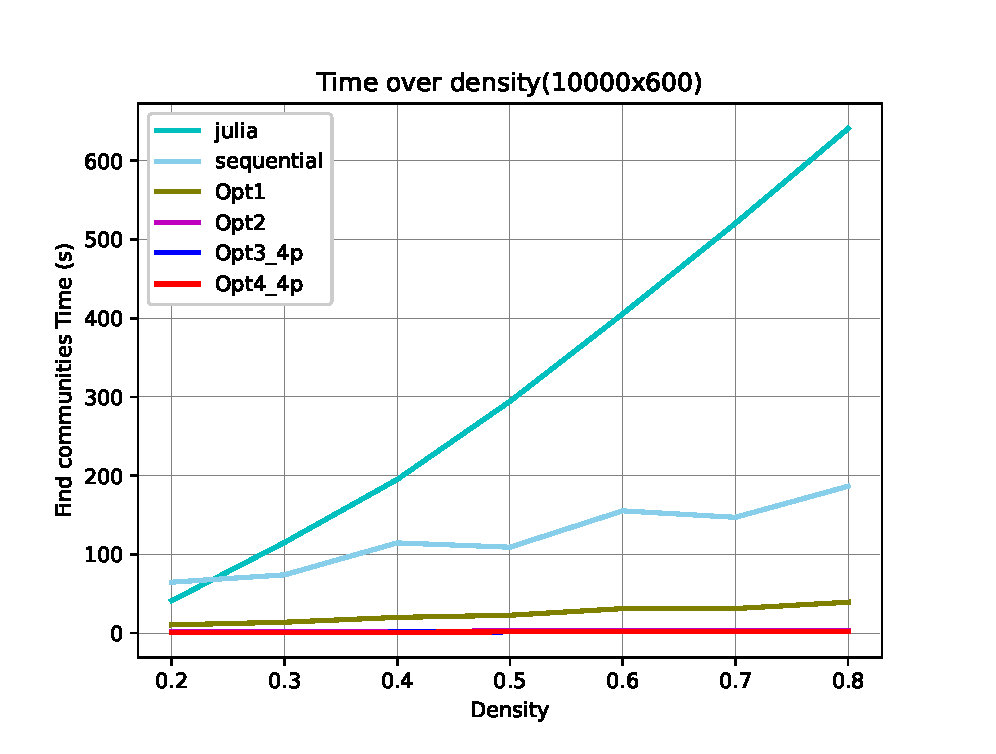
\includegraphics[scale=0.55]{img/timeOverDensityMedium3.eps}
    \vspace*{-8mm}
    \caption{Time over density, all optimizations}
    \label{fig:speedup1}
\end{figure}

\begin{figure}[h!]
    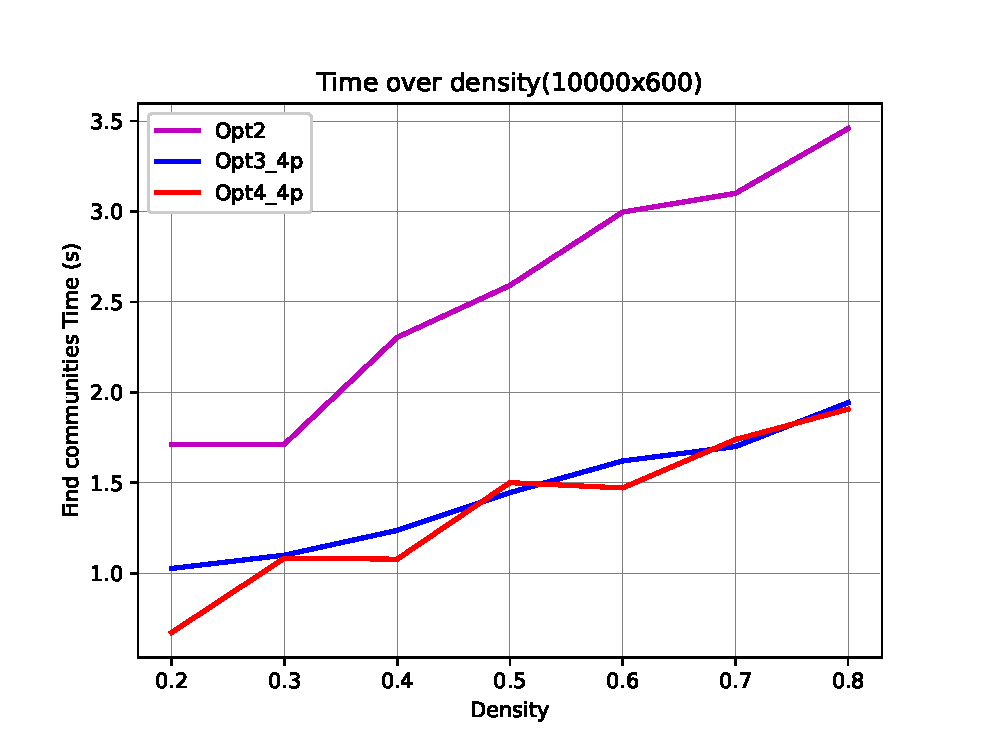
\includegraphics[scale=0.55]{img/timeOverDensityMediumopt234.eps}
    \vspace*{-8mm}
    \caption{Time over density, Opt2, Opt3, Opt4}
    \label{fig:speedup2}
\end{figure}

\mypar{A3}
Looking at the figure \ref{fig:speedup}, the third optimization have a decent scalability from 1 to 2 cores of 1.4, which is slightly below half-way of the optimal result, however it slightly decrease when adding more threads resulting in almost no gain from 3 to 4 threads.
The fourth optimization, instead, showed to not be scalable at all: fro 2 to 4 threads, we had no performance improvement.

\mypar{A4}
These results taken us by surprise: keeping threads on different memory location should have lead to at least a minimum speedup. However, the cause of this failure are not obscure: trying to avoid false sharing, opt4 introduced new data transfers to be handled, because the label vectors were duplicated, and because it was necessary to reorganize the label vectors at the end of each label computation step, we had to remove the \textit{nowait} clause on the two major for loop, introducing some synchronization overhead. It's clear that the trade-off between false sharing\textbackslash data movement was not convenient.

Looking at opt4 we introduce a way higher overhead in the computation, which result in no gains from 1 to 2 cores with some degree of gains from 3 to 4, anyway it doesn't perform any better than opt3.

\begin{figure}[h!]
    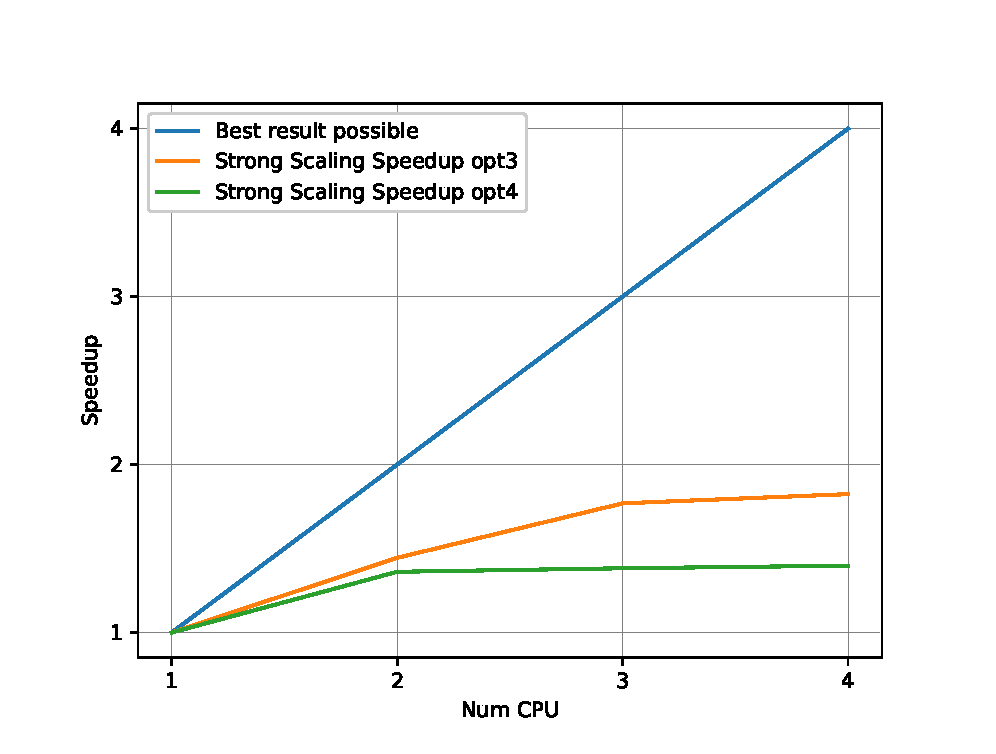
\includegraphics[scale=0.55]{img/speedUP.eps}
    \vspace*{-8mm}
    \caption{Speed-up on size MN - Strong scaling Opt3 and Opt4, 1 to 4 processors}
    \label{fig:speedup}
\end{figure}

\section{Conclusions}

We optimized the Julia version of the Find communities algorithm on Hypergraph porting it to C++, reworking the data structures used and introducing parallelism.
From the base version, we gained a huge absolute speed-up of 196,32 in the best cases.
The poor speed-up obtained with the introduction of parallelism confirmed that obtains good multithread performance on hypergraphs is challenging, and that more detailed studies about parallel algorithm on this structure are required.
However, we showed that only by reworking how the data are memorized and defining \textit{ad-hoc} algorithm solution it is possible to achieve strong improvement in performance and therefore we believe that this should be the main goal of algorithm designer when working with Hypergraphs.


\begin{thebibliography}{1}

\bibitem{Hg_introduction}
Bretto, \emph{A.Hypergraph Theory: An Introduction}.  Springer Publishing Company, Incorporated, 2013.

\bibitem{SimpleHypergraphs}
Antelmi, Alessia, et al. "Analyzing, exploring, and visualizing complex networks via hypergraphs using SimpleHypergraphs. jl." arXiv preprint arXiv:2002.04654 (2020).

\bibitem{LP_standard}
Raghavan, U. N., Albert, R., and Kumara, S. \emph{Near linear time algorithm to detect community structures in large-scale networks}.Physical review. E, Statistical, nonlinear, and soft matter physics 76(2007)

\bibitem{find_community_eigenvectors}
M.E.J.Neman (2006). \textit{Finding community structure in networks using the eigenvectors of matrices}. Phys. Rev. E. 74 (3): 1–19. arXiv:physics/0605087

\bibitem{SystemFrontiers}
Peng, Y., Shi, J., Fantinato, M., and Chen, J. A study on the author collaboration network in big data. Information Systems Frontiers 19, 6 (jun 2017),
1329–1342

\bibitem{PhysicalReview}
Vargas, D. L., Bridgeman, A. M., Schmidt, D. R., Kohl, P. B., Wilcox,
B. R., and Carr, L. D. Correlation between student collaboration network
centrality and academic performance. Physical Review Physics Education Research
14, 2 (oct 2018).

\bibitem{LabelPropagation}
Learning from Labeled and Unlabeled Data with Label Propagation,
Xiaojin Zhu and Zoubin Ghahramani,
School of Computer Science Carnegie Mellon University Pittsburg, PA 15213,
June 2002

% \bibitem{CommunitySearch}
A Survey of Community Search Over Big Graphs
Yixiang Fang · Xin Huang · Lu Qin · Ying Zhang ·
Wenjie Zhang · Reynold Cheng · Xuemin Lin

\bibitem{Julia}
Julia: A Fast Dynamic Language for Technical Computing
Jeff Bezanson, Stefan Karpinski, Viral B. Shah, Alan Edelman
September 25, 2012

\bibitem{OpenMp}
The OpenMP API covers only user-directed parallelization, wherein the programmer explicitly specifies the actions to be taken by the compiler and runtime system in order to execute the program in parallel.
https://www.openmp.org/spec-html/5.1/openmp.html

\bibitem{MarsenneTwister}
Matsumoto, Makoto, and Takuji Nishimura. "Mersenne twister: a 623-dimensionally equidistributed uniform pseudo-random number generator." ACM Transactions on Modeling and Computer Simulation (TOMACS) 8.1 (1998): 3-30.

\bibitem{threadSafeMarsenneTwister}
\emph{The original C implementation of Mersenne Twister is not thread-safe. Here I provide a modification which makes the code thread-safe.}
http://users.umiacs.umd.edu/~yangcj/mtrnd.html

\bibitem{bitset}
The class template bitset represents a fixed-size sequence of N bits. Bitsets can be manipulated by standard logic operators and converted to and from strings and integers.
https://en.cppreference.com/w/cpp/utility/bitset

\bibitem{SH.jl}
A simple hypergraphs package for the Julia programming language.
https://github.com/pszufe/SimpleHypergraphs.jl

\bibitem{community_social}
M. Girvan and M. E. J. Newman, Community structure
in social and biological networks. Proc. Natl. Acad. Sci.
USA 99, 7821–7826 (2002)

\bibitem{community_web}
G. W. Flake, S. R. Lawrence, C. L. Giles, and F. M. Coetzee, Self-organization and identification of Web communities. IEEE Computer 35, 66–71 (2002)


\end{thebibliography}

\end{document}